% Options for packages loaded elsewhere
\PassOptionsToPackage{unicode}{hyperref}
\PassOptionsToPackage{hyphens}{url}
\documentclass[
]{article}
\usepackage{xcolor}
\usepackage[margin=1in]{geometry}
\usepackage{amsmath,amssymb}
\setcounter{secnumdepth}{-\maxdimen} % remove section numbering
\usepackage{iftex}
\ifPDFTeX
  \usepackage[T1]{fontenc}
  \usepackage[utf8]{inputenc}
  \usepackage{textcomp} % provide euro and other symbols
\else % if luatex or xetex
  \usepackage{unicode-math} % this also loads fontspec
  \defaultfontfeatures{Scale=MatchLowercase}
  \defaultfontfeatures[\rmfamily]{Ligatures=TeX,Scale=1}
\fi
\usepackage{lmodern}
\ifPDFTeX\else
  % xetex/luatex font selection
\fi
% Use upquote if available, for straight quotes in verbatim environments
\IfFileExists{upquote.sty}{\usepackage{upquote}}{}
\IfFileExists{microtype.sty}{% use microtype if available
  \usepackage[]{microtype}
  \UseMicrotypeSet[protrusion]{basicmath} % disable protrusion for tt fonts
}{}
\makeatletter
\@ifundefined{KOMAClassName}{% if non-KOMA class
  \IfFileExists{parskip.sty}{%
    \usepackage{parskip}
  }{% else
    \setlength{\parindent}{0pt}
    \setlength{\parskip}{6pt plus 2pt minus 1pt}}
}{% if KOMA class
  \KOMAoptions{parskip=half}}
\makeatother
\usepackage{graphicx}
\makeatletter
\newsavebox\pandoc@box
\newcommand*\pandocbounded[1]{% scales image to fit in text height/width
  \sbox\pandoc@box{#1}%
  \Gscale@div\@tempa{\textheight}{\dimexpr\ht\pandoc@box+\dp\pandoc@box\relax}%
  \Gscale@div\@tempb{\linewidth}{\wd\pandoc@box}%
  \ifdim\@tempb\p@<\@tempa\p@\let\@tempa\@tempb\fi% select the smaller of both
  \ifdim\@tempa\p@<\p@\scalebox{\@tempa}{\usebox\pandoc@box}%
  \else\usebox{\pandoc@box}%
  \fi%
}
% Set default figure placement to htbp
\def\fps@figure{htbp}
\makeatother
\setlength{\emergencystretch}{3em} % prevent overfull lines
\providecommand{\tightlist}{%
  \setlength{\itemsep}{0pt}\setlength{\parskip}{0pt}}
\usepackage{bookmark}
\IfFileExists{xurl.sty}{\usepackage{xurl}}{} % add URL line breaks if available
\urlstyle{same}
\hypersetup{
  pdftitle={Practice Midterm Examination},
  pdfauthor={Jaye Seawright},
  hidelinks,
  pdfcreator={LaTeX via pandoc}}

\title{Practice Midterm Examination}
\usepackage{etoolbox}
\makeatletter
\providecommand{\subtitle}[1]{% add subtitle to \maketitle
  \apptocmd{\@title}{\par {\large #1 \par}}{}{}
}
\makeatother
\subtitle{Political Science 210 --- Fall 2026}
\author{Jaye Seawright}
\date{Practice for October 29 review --- Fall 2026}

\begin{document}
\maketitle

\vspace{1cm}

\textbf{About this practice exam:} This is built to the same
specification as the real midterm --- nine questions, 100 points plus 2
extra credit, 75 minutes, the same point distribution, and the same
kinds of questions. Only the studies are different. Both studies here
are ones we have discussed in class, so you should be able to focus on
the \emph{skills} the exam tests rather than on decoding unfamiliar
material.

\textbf{Instructions (as they will appear on the real exam):} This exam
is \textbf{open notes but closed devices}. You may consult your own
handwritten or printed notes. No laptops, phones, tablets, or any
electronic devices are permitted. The figures and tables you need are
printed on the following pages. \textbf{Write your answers in the spaces
provided below each question.} You have 75 minutes.

The exam has 9 questions worth a total of \textbf{100 points}. Point
values are shown in brackets.

If you find ambiguity in a question, adopt a reasonable reading, note
your assumption briefly, and proceed.

\newpage

\section{Figures and Tables for Study
1}\label{figures-and-tables-for-study-1}

\newpage
\begin{figure}

{\centering 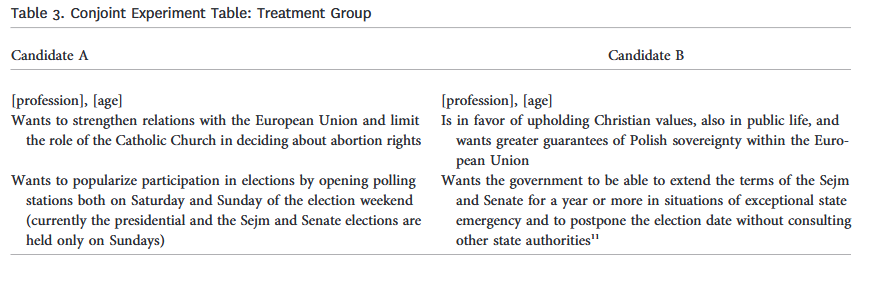
\includegraphics[width=0.95\linewidth]{img/pm_chiopris_table3} 

}

\caption{**Table 3 (Chiopris, Nalepa & Vanberg)** – The paired-candidate vignette shown to the treatment group.}\label{fig:chiopris-table3}
\end{figure}

\newpage
\begin{figure}

{\centering 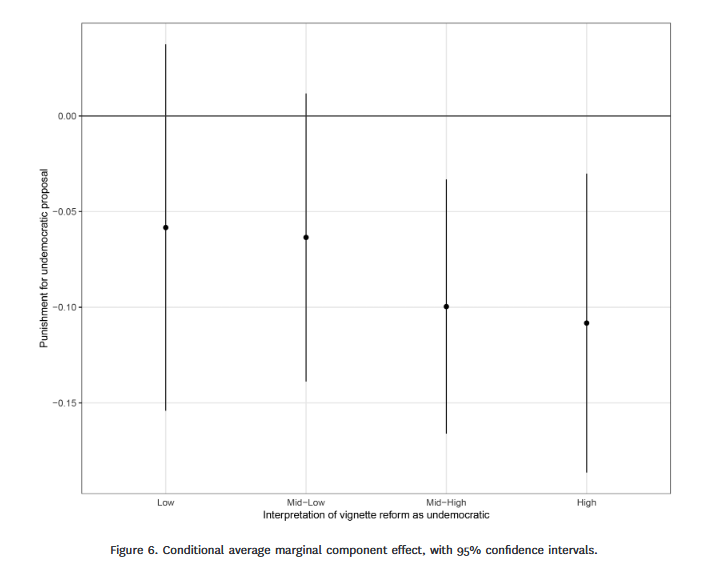
\includegraphics[width=0.8\linewidth]{img/pm_chiopris_fig6} 

}

\caption{**Figure 6 (Chiopris, Nalepa & Vanberg)** – Conditional average marginal component effect of the undemocratic proposal on punishment, by how undemocratic respondents judged the reform to be. Bars are 95 percent confidence intervals.}\label{fig:chiopris-fig6}
\end{figure}

\newpage
\begin{figure}

{\centering 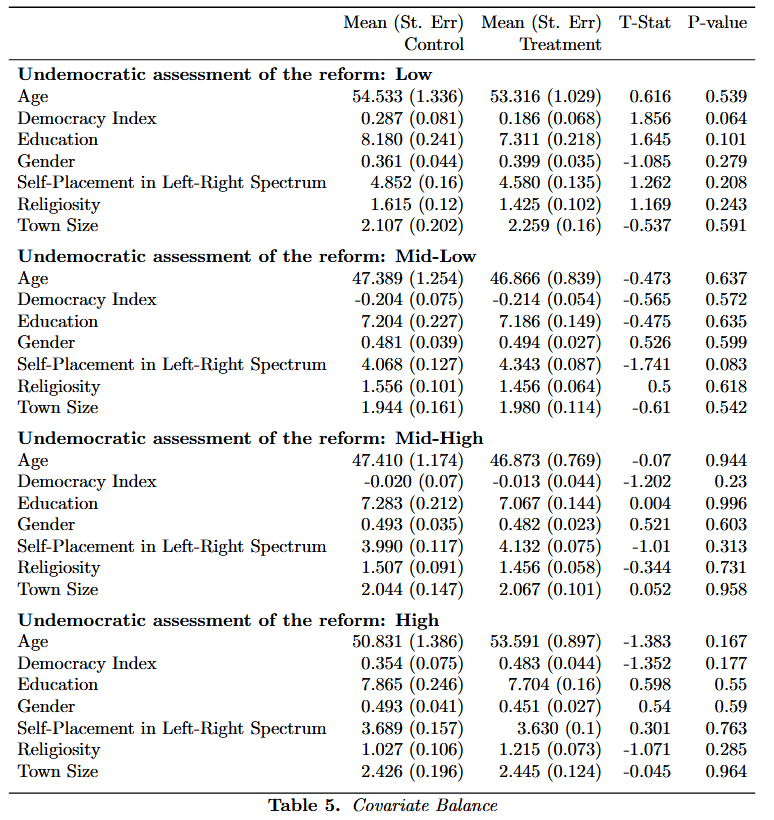
\includegraphics[width=0.85\linewidth]{img/pm_chiopris_table5} 

}

\caption{**Table 5 (Chiopris, Nalepa & Vanberg)** – Covariate balance between control and treatment groups, within each level of perceived undemocratic assessment.}\label{fig:chiopris-table5}
\end{figure}

\newpage

\section{Figures and Tables for Study
2}\label{figures-and-tables-for-study-2}

\emph{Bhavnani, ``Do Electoral Quotas Work after They Are Withdrawn?
Evidence from a Natural Experiment in India.''}

\textbf{Background.} Seats on the Mumbai city council were
\textbf{reserved for women by lottery}, one election at a time. Bhavnani
compares wards that were reserved in 1997 and then open again in 2002
against wards that were open in both years, asking whether women kept
winning after the quota was withdrawn.

\newpage
\begin{figure}

{\centering 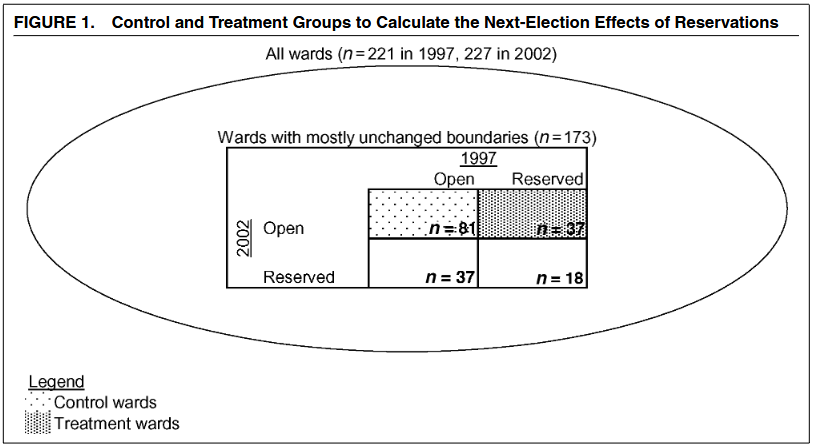
\includegraphics[width=0.8\linewidth]{img/pm_bhavnani_design} 

}

\caption{**Figure 1 (Bhavnani)** – The research design. Treatment wards were reserved in 1997 and open in 2002; control wards were open in both years.}\label{fig:bhavnani-design}
\end{figure}

\newpage
\begin{figure}

{\centering 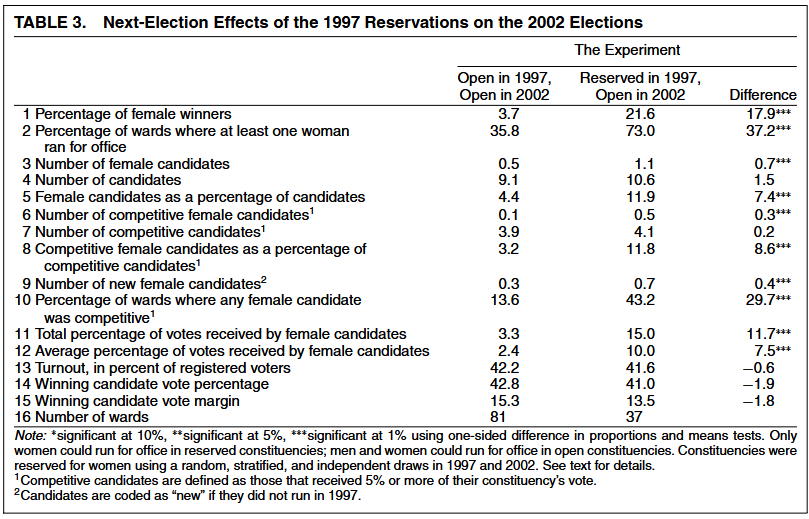
\includegraphics[width=0.95\linewidth]{img/pm_bhavnani_table3} 

}

\caption{**Table 3 (Bhavnani)** – Next-election effects of the 1997 reservations on the 2002 elections.}\label{fig:bhavnani-table3}
\end{figure}

\newpage

\section{Exam Questions}\label{exam-questions}

\subsection{Study 1: Citizen Uncertainty and Democratic Backsliding (40
points)}\label{study-1-citizen-uncertainty-and-democratic-backsliding-40-points}

\emph{Chiopris, Nalepa \& Vanberg study whether Polish voters punish
candidates who propose undemocratic reforms. Respondents read a pair of
candidate profiles; in the treatment condition, one candidate proposes
extending parliamentary terms and postponing elections during a state of
emergency.}

\textbf{Question 1} (12 points) (a) What is the \textbf{treatment} in
this study? Be specific about how it is delivered to respondents. What
is the \textbf{outcome} being measured?

\begin{enumerate}
\def\labelenumi{(\alph{enumi})}
\setcounter{enumi}{1}
\tightlist
\item
  The authors also measure how undemocratic each respondent judged the
  proposed reform to be, on a four-category scale from Low to High. Do
  you think this is a valid measure of that concept? Why or why not?
\end{enumerate}

\vspace{4cm}

\begin{center}\rule{0.5\linewidth}{0.5pt}\end{center}

\textbf{Question 2} (10 points) What kind of \textbf{research design}
does this study use (using the categories discussed in class)? What are
the main strengths and weaknesses of this design for making
\textbf{causal} claims about whether voters punish undemocratic
proposals?

\vspace{4cm}

\begin{center}\rule{0.5\linewidth}{0.5pt}\end{center}

\textbf{Question 3} (10 points) Look at \textbf{Chiopris's Table 5}.

\begin{itemize}
\tightlist
\item
  What is this table for? What does it establish?
\item
  Name \textbf{two threats} to the study's conclusions that covariate
  balance does \textbf{not} address, and explain why balance cannot rule
  them out.
\item
  Two of the comparisons in the table have p-values below 0.10
  (Democracy Index in the Low group, and Left--Right Self-Placement in
  the Mid-Low group). Does this undermine the authors' claim that the
  groups are balanced? Explain.
\end{itemize}

\vspace{4cm}

\begin{center}\rule{0.5\linewidth}{0.5pt}\end{center}

\textbf{Question 4} (8 points) Look at \textbf{Chiopris's Figure 6}.

\begin{itemize}
\tightlist
\item
  For which subgroup is the estimated punishment largest in absolute
  magnitude? Approximately what is that estimate?
\item
  Is the estimate for the \textbf{``Low''} subgroup statistically
  significant? How can you tell?
\item
  Do all four subgroups show an effect in the same direction? What does
  the pattern across subgroups suggest?
\end{itemize}

\vspace{4cm}

\begin{center}\rule{0.5\linewidth}{0.5pt}\end{center}

\subsection{Study 2: Electoral Quotas After They Are Withdrawn (60
points)}\label{study-2-electoral-quotas-after-they-are-withdrawn-60-points}

\emph{Seats on the Mumbai city council were reserved for women by
lottery, one election at a time. Bhavnani compares wards reserved in
1997 and open again in 2002 (treatment, n = 37) against wards open in
both years (control, n = 81).}

\textbf{Question 5} (10 points)\\
What kind of \textbf{research design} is this (be specific)? Pay
attention to \textbf{who} carried out the randomization. What are the
main advantages and disadvantages of this design for descriptive and
causal inference?

\vspace{4cm}

\begin{center}\rule{0.5\linewidth}{0.5pt}\end{center}

\textbf{Question 6} (8 points)\\
What is the \textbf{treatment} in this study, and what are its two
levels? What is the \textbf{unit of analysis} --- what is being compared
to what?

\vspace{3cm}

\begin{center}\rule{0.5\linewidth}{0.5pt}\end{center}

\textbf{Question 7} (12 points)\\
Look at \textbf{Bhavnani's Table 3}.

\begin{itemize}
\tightlist
\item
  In row 1, what percentage of control wards and what percentage of
  treatment wards elected a female winner in 2002? Roughly how many
  times larger is the treatment figure?
\item
  Which row shows the largest difference between treatment and control?
  What is that difference?
\item
  How can you tell from the table which differences are statistically
  significant?
\end{itemize}

\vspace{4cm}

\begin{center}\rule{0.5\linewidth}{0.5pt}\end{center}

\textbf{Question 8} (15 points)\\
Still in \textbf{Bhavnani's Table 3}, look at rows 4, 7, 13, 14, and 15
--- number of candidates, number of competitive candidates, turnout,
winning candidate vote percentage, and winning candidate vote margin.

\begin{itemize}
\tightlist
\item
  What do these five rows have in common, and how do they differ from
  rows 1, 2, and 11?
\item
  Why would an author \emph{want} to report rows like these, even though
  they show no effect?
\item
  What would it have meant for the study's conclusions if row 13
  (turnout) had shown a large and significant difference?
\end{itemize}

\vspace{5cm}

\begin{center}\rule{0.5\linewidth}{0.5pt}\end{center}

\textbf{Question 9} (15 points)\\
Bhavnani concludes that reservations have effects that \textbf{persist
after the quota is withdrawn}.

\begin{itemize}
\tightlist
\item
  Using Bhavnani's Table 3, how well supported is that conclusion? Cite
  specific rows.
\item
  The design compares wards reserved in 1997 against wards never
  reserved. What does the lottery accomplish that a simple comparison of
  reserved and unreserved wards could not?
\item
  What additional evidence would you want before accepting that quotas
  would have similar lasting effects elsewhere?
\item
  \textbf{Bonus (2 extra points):} Row 2 shows that 73.0 percent of
  treatment wards had at least one woman run, against 35.8 percent of
  control wards. Why might this row matter more than row 1 for
  understanding \emph{why} the quota had lasting effects? (Write your
  answer in the space below.)
\end{itemize}

\vspace{5cm}

\begin{center}\rule{0.5\linewidth}{0.5pt}\end{center}

\textbf{End of practice exam.} \emph{Total points: 100 (plus up to 2
extra credit).}

\vspace{0.5cm}

\textbf{Note:} On the real exam you will write your answers on the exam
paper and hand it in before leaving.

\end{document}
